% L'option handout permet de supprimer la barre de navigation
\documentclass[handout]{beamer}
\usepackage[utf8]{inputenc}
\usepackage[french]{babel}
\usepackage[T1]{fontenc}
\usepackage{amsmath}
% Pour pouvoir insérer des images
\usepackage{graphicx}
\usepackage{wrapfig}
\graphicspath{images/}
% Gestion des couleurs
\usepackage{color}
\definecolor{red}{RGB}{231, 76, 60}

% Un joli thème flat
\usetheme{Rochester}

% Personnalisation du thème
\usecolortheme[named=red]{structure}
% Numéro de slides dans le footer
\setbeamertemplate{footline}[frame number]
\setbeamertemplate{blocks}[shadow=false]

% ------------------------------------ %
% -- METADONNÉES DU DOCUMENT --------- %
\title{
	A quad-tree approach to image segmentation which combines statistical and spatial information
}
\author{
	Manon \textsc{Ansart} \\
	\vspace{5px}
	Antoine \textsc{Augusti}
}
\date{7 janvier 2015}

% Générer une page de titre à chaque début de section
\AtBeginSection[]
{
	\begin{frame}[plain]
	\frametitle{Sommaire}
	\tableofcontents[currentsection, hideothersubsections]
	\end{frame}
}

% Début du document
\begin{document}

	% Génération de la page de titre
	\begin{frame}[plain]
		\titlepage
	\end{frame}

	% Génération du sommaire
	\begin{frame}[plain]
		\frametitle{Sommaire}
		\tableofcontents
	\end{frame}


	% //////////////////////////////// %
	% /// La segmentation //////////// %
	\section{La segmentation}

		%% Principe général
		\subsection{Principe général}
		\begin{frame}
			\frametitle{Principe général}

			La segmentation est une opération qui a pour but de rassembler des pixels entre eux suivant des critères pré-définis.\\
			\vspace{10px}
			\textbf{Segmentation statistique}
			\begin{itemize}
				\item Par seuillage : choix de plusieurs seuils pour assigner une classe à chaque pixel. Maximisation de l'entropie, méthode d'Otsu\dots
				\item Par classification : algorithme des K-moyennes par exemple.
			\end{itemize}

			\vspace{10px}
			\textbf{Segmentation spatiale}
			\begin{itemize}
				\item Approche par croissance de région ou par décomposition / fusion.
			\end{itemize}

		\end{frame}

	% ///////////////////////////// %
	% /// L'algorithme //////////// %
	\section{L'algorithme}

		%% Le quadtree
		\subsection{Le quadtree}
		\begin{frame}
			\frametitle{Le quadtree}

			Un quadtree région ayant une profondeur $n$ peut être utilisé pour représenter une image de $2^n \times 2^n$ pixels, où la valeur de chaque pixel est 0 (noir) ou 1 (blanc). Chaque nœud possède 4 fils.
			\begin{figure}[H]
				\centering
				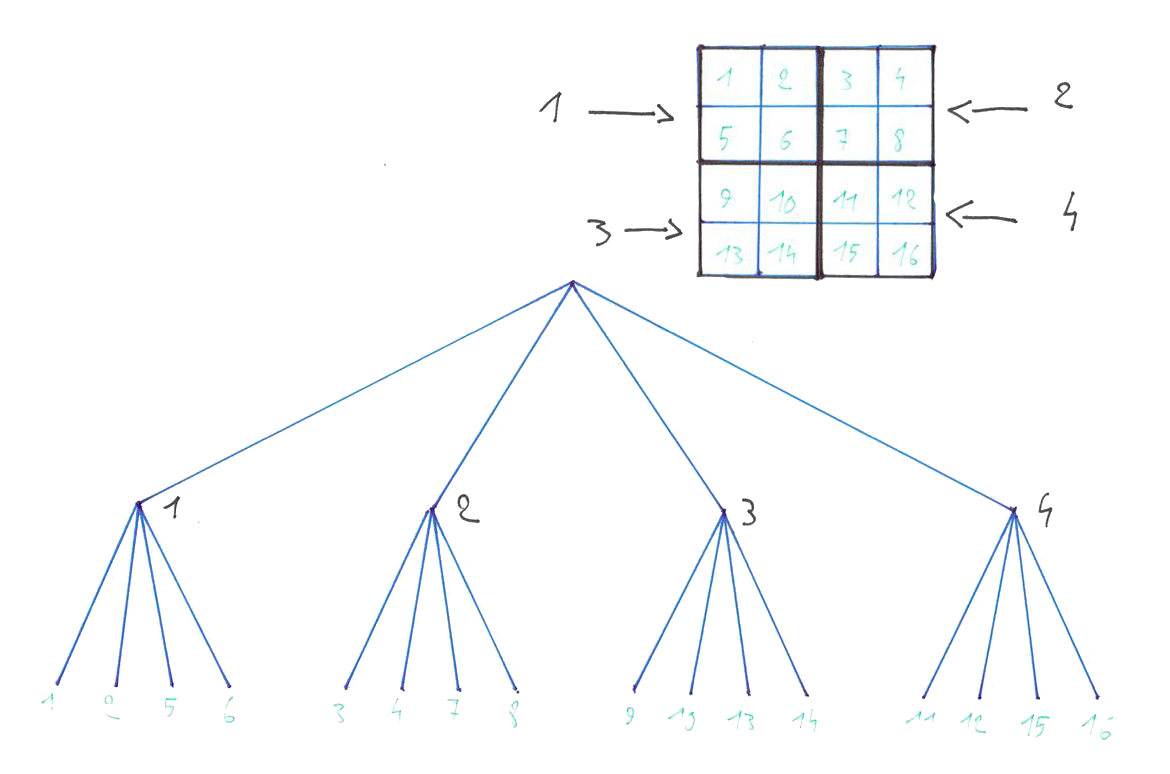
\includegraphics[scale=0.19]{images/quadtree-dessin.jpg}
				\caption{Représentation d'un quadtree.}
				\label{fig:quadtree2}
			\end{figure}
		\end{frame}

		%% Le lissage
		\subsection{Le lissage}
		\begin{frame}
			\frametitle{Le lissage}
				\begin{itemize}
					\item Utilisation d'un quadtree pour lisser l'image. Quand le rang du quadtree augmente, l'image est lissée (chaque pixel a pour valeur la moyenne de 4 autres) ;
					\item Recherche d'un niveau optimal $m'$ pour lequel le lissage est suffisant pour effectuer la segmentation.
				\end{itemize}

				On veut trouver les régions de rayon minimal $r = 2^n$, tout en lissant l'image le plus possible, c-à-d en maximisant $m'$.

				\[2^{m' + 1} \leq 2^n \Leftrightarrow m'+1 \leq n \Leftrightarrow m' \leq n - 1\]
				On obtient le problème d'optimisation :
				\begin{equation*}
				\begin{aligned}
					& \underset{m' \in\; [0; n]}{\text{max}}
					& & m' \\
					& \text{Sous contrainte}
					& & m' \leq n - 1
					\end{aligned}
				\end{equation*}
		\end{frame}

		%% Classification statistique
		\subsection{Classification statistique}
		\begin{frame}
			\frametitle{Classification statistique}
				\begin{itemize}
					\item Utilisation de l'algorithme du barycentre local ;
					\item Pas de connaissance a priori du nombre de régions ;
					\item Seul paramètre : taille de la fenêtre. Peut être supprimé grâce à un processus itératif ;
					\item Classification effectuée une fois que l’algorithme du barycentre local a convergé.
				\end{itemize}
		\end{frame}

		%% Estimation de la frontière
		\subsection{Estimation de la frontière}
		\begin{frame}
			\frametitle{Estimation de la frontière}
				\begin{itemize}
					\item Identification de la frontière : Les nœuds dont un voisin est d'une classe différente appartiennent à $B$, les nœuds dont un voisin appartient à $B$ appartiennent à $B_1$ ;
					\begin{figure}[H]
						\centering
						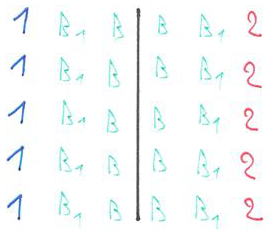
\includegraphics[scale=0.19]{images/bordure-3.jpg}
						\caption{Identification de la frontière sur une ligne droite.}
						\label{fig:quadtree2}
					\end{figure}
					\item Lissage de la frontière avec un filtre linéaire;
					\item Réaffectation de la classe ayant la moyenne la plus proche aux pixels de la frontière;
					\item Répétition à tous les niveaux du quadtree.
				\end{itemize}
		\end{frame}

	% //////////////////////////////// %
	% /// Conclusion //////////// %
	\section{Conclusion}

		\begin{frame}
			\frametitle{Conclusion}
			Les méthodes de segmentation statistique et spatiale décrites en introduction prennent en compte différents paramètres et se complètent. La spécificité de l'algorithme présenté est qu'il combine les deux techniques :
			\begin{itemize}
				\item Approche statistique : classification à l'aide de l’algorithme du barycentre local ;
				\item Approche spatiale : Travail sur la frontière avec d'identification et le filtre.
			\end{itemize}
		\end{frame}

\end{document}